\documentclass[a4paper]{article}

\usepackage[english]{babel}
\usepackage[utf8x]{inputenc}
\usepackage{amsmath}
\usepackage{graphicx}
\usepackage{hyperref}

\usepackage[colorinlistoftodos]{todonotes}
\usepackage[left=1in,right=1in]{geometry}
\title{CS 387 Database and Information Systems Lab\\
Project Proposal - ConsumerConnect}
\author{
Astha Agarwal (110050018)\\
Anmol Garg (110050020)\\
Deepali Adlakha (11D170020)}

\begin{document}
\maketitle


\section{Introduction - Application Domain}


As our CS 387 project, we have planned to make an online service portal, whereby people can interact with service providers and other customers to seek opinion and decide the appropriate service provider/service they want to use. Here, 'customers' refer to other users on the database, who also interact in a similar manner.\\On the other side, service providers will also be able to interact with users to know their potential customers. They can give details about the services they provide, and answer customer queries.\\The project involves crowdsourcing, search and social networking.

\section{Functional Specification}

Broadly, there are two types of users of our application - customers and service providers. We plan to provide a portal for them to interact. 
At present, we have not added any administrators, though this is a feature that can be added if required. Here is a brief description of the facilities which will be provided to the users:

\subsection{Customer}
\begin{enumerate}
\item \textbf{Personal Details -} Users can provide their personal information like name, address, age, gender etc. 
\item \textbf{Reviews - }Users can provide reviews and rate the service providers according to their experience. (Validating the experience can be seen as a further extension of the project.) Also, they can upvote ot downvote others' reviews. Users will earn points when their reviews are upvoted. Their rank improves as the number of points increases.
\item \textbf{Friends - }Users can see the details of other users tagged as friends and reviews posted by them.
\item \textbf{Messaging - }Users can send a message to other customers to seek opinion or otherwise.
\item \textbf{Past Experiences - }User can refer to his experience in the past, and make an informed decision accordingly.
\item \textbf{Wishlist - }User can maintain a wishlist of the services required by him for future reference.
\item \textbf{Appointments - } Customers can book an appointment with a service provider for a particular service. 
\item \textbf{Bidding - } The wishlist of customers can be viewed by a service provider, and he can post a bid for the corresponding service. Customer can then make a decision by comparing various prices and options depending on the response of service providers.

\end{enumerate}

\subsection{Service Provider}
\begin{enumerate}
\item \textbf{Provider Details - }Users can provide their personal information like name, address, age, gender etc.
\item \textbf{Service Details - }User can add the details of service provided by him such as service type, rates, availability etc. 
\item \textbf{Rating - }An average rating based on reviews given by customers to his services.
\item \textbf{Reviews - }The reviews given by his customers will be visible to other willing customers for reference.
\item \textbf{Bidding and Appointments - } As explained above, these are interactions between service providers and customers, which help them communicate well with each other.

\end{enumerate}


\section{Data Model Specification}

In our ER Model Diagram, in addition to the popular convention, we have used separate colour for the weak relationship sets 

\subsection{Entities}

\begin{enumerate}
\item \textit{User} of our application - The user has been allotted a User ID
Login ID, Password, Name, E-mail ID, Photograph and Contact Number. Two entities are inherited from the \textit{User - Customer} and \textit{Service Provider}.
\item \textit{Customer}, is one possible profile for a \textit{User} and is alloted a customerID (Primary Key). The customer has a Gender, Date of Birth, Age, (derived attribute), Cumulative Points (earned through the votes on his reviews to Services) and Rank (derived from his Cumulative Points).

\item \textit{Service Provider}, is the second possible profile for the \textit{User} and is allotted a Service Provider ID (Primary Key). \textit{Service Provider} has a Rating, a quantitative measure of the quality of services he provides. (derived attribute). He can also mention his Webpage.
 
\item \textit{Service} - It has a Service ID(Primary Key) and Name. The Type of Service is a broad categorisation (eg. Doctor, Repair) and Sub-Type is a specific category(eg. Cardiology, Cycle Repair). There can be a Mini Description associated to the service.

\item \textit{Review}, given by a \textit{Customer} to a \textit{Service} provided by a \textit{Service provider}. It has a primary key Review ID. There is a Content of the Review, a Rating which the customer gives to the service (and service provider), and a timestamp showing when the review was posted.

\item \textit{Wish -} Also has a Wish ID(Primary Key), a Description (if the customer wants to add any general comments related to the Service he wants). There can be a specific Requirement period, (composite attribute) that contains Time, Day and Month when the customer wants to use the Service. He can also add a Maximum Price that he is willing to pay in return of the \textit{Service} offered.

\item \textit{Location -} To describe the location, following entities are used: \textit{Street, City, State and Country}. They contain names of the respective entities.

The following entities are used for the interaction between the Service Provider and the Customer:

\item \textit{Question} is put up by the \textit{Customer} to be answered subsequently by the \textit{Service Provider}. It has a Question ID(Primary Key), Description and Timestamp (when the question was raised).

\item \textit{Answer} is put up by the \textit{Service Provider} in response to a \textit{Question}. It has an Answer ID (Discriminating Key), Description (content of the Answer) and Timestamp.

\end{enumerate}
\subsection{Relationships}

\begin{enumerate}
\item \textit{Provides - Service Provider} provides a \textit{Service} at a \textit{Street} in a \textit{City} in a \textit{State} in a \textit{Country}. It includes the Availability (a composite attribute containing Time, Day and Month) so that customers can book appointments, Description, Price (Cost incurred on the Service) and the Discount offered (if any). Note that a \textit{Service Provider} can provide multiple services of the same type and different subtypes.

\item \textit{Experience -} A \textit{Customer} experiences a \textit{Service} and puts a \textit{Review} on it.

\item \textit{Vote}, Up/Down vote by a \textit{Customer} to a \textit{Review}
\item \textit{Wishes - Service} wanted by a \textit{Customer}

\item \textit{Lives}, a \textit{Customer} lives in a \textit{Street} in a \textit{City} in a \textit{State} in a \textit{Country}
\item \textit{Q\&A}, \textit{Question} raised by a \textit{Customer} to a \textit{Service Provider} and the subsequent \textit{Answer}
\item \textit{Friend}, A \textit{Customer} is a friend of another \textit{Customer}
\item \textit{Message}, sent by a \textit{Customer} to a \textit{Customer}
\item \textit{Bids -} A \textit{Service Provider} offers to fulfil a \textit{Customer's} Wish at a particular price, that is the Bid Value. It may also contain a small Description.
\item \textit{Appointment -} A \textit{Customer} books an appointment for a particular \textit{Service} to be offered by a \textit{Service Provider} at a Location alongwith the details of the Appointment that includes the Scheduled time and Cost of the \textit{Service}.
\end{enumerate}


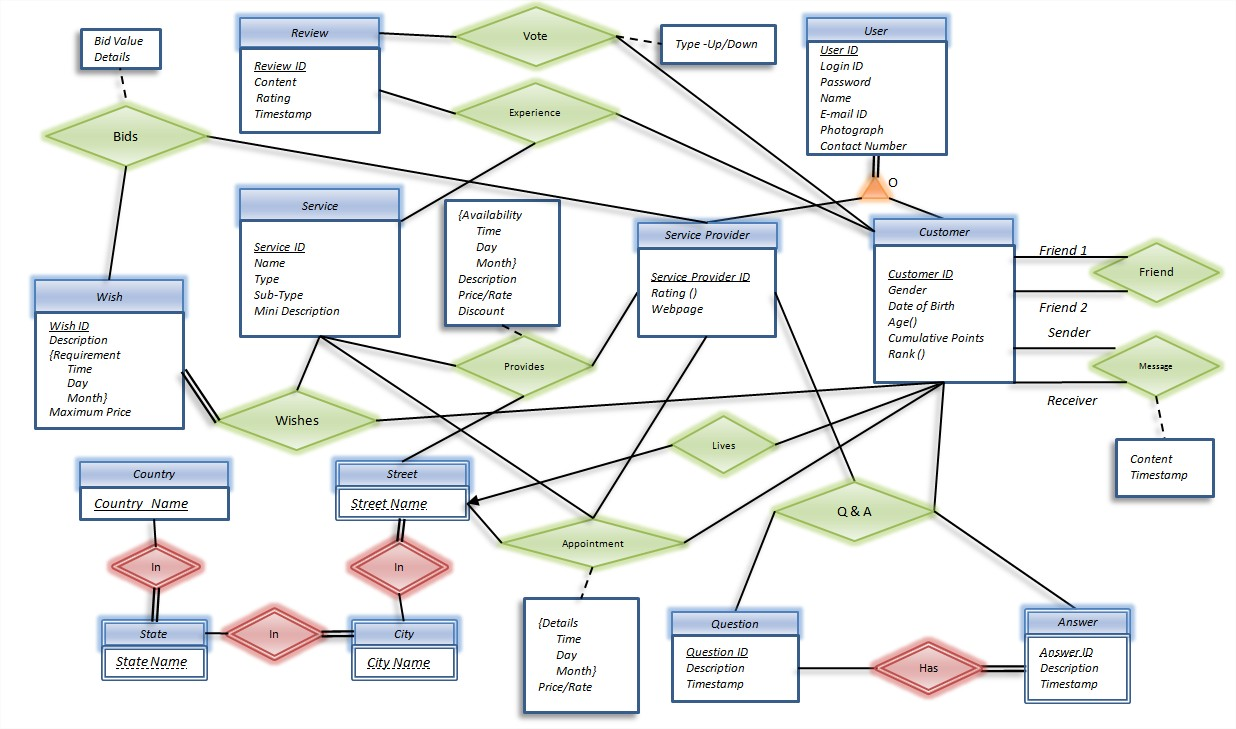
\includegraphics[width=160mm]{ermodel.jpg}
\section{Test Plan}

\subsection{Data}
For our application, the data would be generated randomly by a program or online by crawling a website. To test our application, we will manually generate SQL queries corresponding to the above functionalities and test it against the data collected.

\subsection{Functionalities (provided to the customer)}
\begin{enumerate}
\item Looking out for a service at a particular location, with a particular availability - by putting filters on services. He can also see the reviews provided by other people for that service.
\item Select a service by a service provider, review it and earn points for the same - Review must be properly linked to the service provider and his service. There cannot be a review for a service that does not exist.
\item Asking questions to a service provider which are subsequently answered by the service provider.
\item Interacting with other customers via personal messages - Message must go to only the cutomer inteded.
\item UpVote/DownVote someone else's review on the basis of his own experience - Now, we have to store who upvoted which answer, and not to allow multiple upvotes on same answer by same user.
\item The customer can view his friend list, and reviews provided by them.
\item Book an Appointment on the basis of the Availability of the Service - A service can be booked only if it is available for the time period required by the customer.
\end{enumerate}

\subsection{Functionalities (provided to the customer)}
\begin{enumerate}
\item Put out details of the services provided by him. HE can also offer discounts.
\item The Service Provider can get to see the customers who are interested in taking up his service (through their wishlist) and the maximum price they can pay for it, therefore he can take selective decisions to increase his customer base.
\item Can answer questions posted to him by the customers.
\end{enumerate}

The above features are offered by our application. For search/querying, we will also be adding the option to order results by availability / discounts / price etc. This can directly be handled by 'order by' option provided by SQL.



\section{Future Extensions}
Other than the above mentioned, we will aim to model the following aspects if time permits. 

\begin{enumerate}
\item \textbf{Customisation based on kind of service -} Depending on the kind of service one provides, he might want to have a customised profile through which he can properly showcase the facilities available to him. But at present, we are keeping a general information area for the same.
\item \textbf{Authentication of Service Provider -} How to know whether a service provider actually exists, or is it fake profile?
\item \textbf{Authentication of Reviews -} Did the customer actually receive a service? Or is he providing fake reviews (Note that this is partly handled by the concept of customer rating which we are including in the project.)
\item \textbf{Followers of a Service Provider - }We have also thought of the concept of "following" a service provider, i.e. receive his updates, reviews etc. via notifications.
\item \textbf{Integration with Social Platforms - }We can integrate it with existing social networks like Twitter, Facebook etc.
\end{enumerate}


\section{Relational Model}

\subsection{For Entity Sets}
Assuming E/R Model Approach for hierarchy relationship in Users (Customer, ServiceProvider):

\begin{enumerate}

\item User(\underline{UserID}, LoginID, Password, FirstName, LastName, EmailID, Photograph, ContactNumber)

\item Customer(\underline{UserID}, Gender, DOB, Age, CumulativePoints, Rank)

\item ServiceProvider(\underline{UserID}, Rating, Webpage)

\item Service(\underline{ServiceID}, Name, Type, SubType, MiniDescription)

\item  \textbf{Many-to-Many Bad Relational Design -}\\  Review(\underline{ReviewID}, Content, Rating, TimeStamp, \underline{VotedByCustomerUserID}, TypeOfVote)

\item Wish(\underline{WishID}, Description, MaximumPrice);

\item WishTime(\underline{WishID, StartTime}, EndTime);

\item Question(\underline{QuestionID}, Description, TimeStamp);

\item Answer(\underline{QuestionID, AnswerID}, Description, TimeStamp);

\item Country(\underline{CountryName}); 

\item State(\underline{CountryName,StateName});

\item City(\underline{CountryName,StateName,City});

\item \textbf{Many-to-One Bad Relational Design- } \\ Street(\underline{CustomerUserID, StreetName, CityName, StateName, CountryName}) 
\end{enumerate}


\textbf{Note:} 
\begin{enumerate}
\item We have removed the CustomerID and ServiceProviderID, as they were redundant in providing unique identification to a type of user. In the E/R approach, we are anyway storing the UserID in Customer and ServiceProvider tables, and hence no need for another unique attribute.
\item We assume that there are no two end times for same start time, thus we haven't considered it as a primary key.
\item For the Many to Many relationship Votes from Review to Customer, we have added CustomerId as the attribute of Review, whereas there should be another relation relating Customer and Review for Votes. In this case, Review Information will be repeated and there can be an issue of consistency. 
\item For the Many to One relationship Lives from Customer to Street, we have added the CustomerID to Street as an attribute. This will not only lead to repetition of information and hence wastage of resources, but also create another problem. We have a ternary relation from ServiceProvider and Service to Street. \\Now we will have to map one location of a service given by a service provider to all tuples corresponding to every customer living at that location, which not only wastes space, but will also complicate search and other functions. So, in the relation for relationships, we have not considered this model, but the correct model which assumes that there is no CustomerID in Street table.

\end{enumerate}


For \textbf{OO Approach}, we have 3 relations again:

\begin{enumerate}
\item CustomerUser(UserID, LoginID, Password, Name, EmailID, Photograph, ContactNumber, Gender, DOB, Age, CumulativePoints, Rank)
\item ServiceProviderUser(UserID, LoginID, Password, Name, EmailID, Photograph, ContactNumber, Rating, Webpage)
\item CustomerServiceProviderUser(UserID, LoginID, Password, Name, EmailID, Photograph, ContactNumber, Gender, DOB, Age, CumulativePoints, Rank, Rating, Webpage)

\end{enumerate}

\newpage
\textbf{Note:} 
\begin{enumerate}

\item Here, there is no table for only User, because user has total participation in the "is a" relationship, and has at least one role as a Customer and/or a ServiceProvider. We note that in this case as well, separate CustomerID and ServiceProviderID are not required to distinguish entries. So, we have removed the two attributes from the relations.
\item Another point to note here is the problem associated with this structure. Suppose there is a User, who has only a customer profile. He starts offering a service and then he makes a service provider profile associated to the same account. In that case, we have to shift all his details from CustomerUser table to CustomerServiceProviderUser table. This might be a cumbersome task. Also, there is no authority that dictates that UserIDs cannot be same in the three tables.

\end{enumerate}


\subsection{For Relationship Sets}

\begin{enumerate}
\item Friend(\underline{CustomerUserID1,CustomerUserID2})
\item Message(\underline{SenderCustomerUserID, ReceiverCustomerUserID}, Content, Timestamp)
\item Experience(\underline{CustomerUserID, ReviewID, ServiceID})
\item Bids(\underline{ServiceProviderUserID, WishID}, BidValue, Details)
\item Wishes(\underline{CustomerUserID, WishID,ServiceID})
\item Provides(\underline{ServiceProviderID, ServiceID, StreetName, CityName, StateName, CountryName}, Description, Rate, Discount)
\item ProvideTime(\underline{ServiceProviderUserID, ServiceID, StartTime}, EndTime)
\item Appointment(\underline{CustomerUserID, ServiceID, ServiceProviderUserID, StreetName, CityName},\\ \underline{ StateName, CountryName}, Rate, StartTime,EndTime)  
\item QAndA(\underline{CustomerUserID, ServiceProviderUserID, QuestionID,AnswerID})

\end{enumerate}




\subsection{Foreign Keys}
\begin{enumerate}
\item CustomerUserID and ServiceProviderUserId in any relation are foreign keys into UserID in Users.
\item ServiceID in any relation is foreign key into ServiceID in Services.
\item ReviewID in Experience is foreign key into ReviewID in Reviews.
\item WishID in Wishes, Bids and WishTime are foreign keys into WishID in Wish.
\item QuestionID in Answer is foreign key into QuestionID in Question.
\item QuestionID, AnswerID in QAndA are foreign keys into QuestionID, AnswerID in Answer.
\item For location names, CountryName is a foreign key into Country, StateName is a foreign key into State and CityName is a foreign key into City.
\end{enumerate}



\subsection{Functional Dependencies}
\begin{enumerate}
\item As is obvious, all super keys determine the entire tuple. 
\item Functional dependencies for derived attributes:
\begin{enumerate}
\item In User relation: LoginID $\to$ Password, EmailID $\to$ LoginID, Email-ID $\to$ UserID (In fact, LoginID and emailID are candidate keys)
\item In Customer relation: DOB $\to$ Age,  CumulativePoints $\to$ Rank
\end{enumerate}
\end{enumerate}

\subsection{Assertions}
\begin{enumerate}
\item In case of Appointments, the Start Time and the End Time should be ahead in the future (that is later than the Current time).
\item At the time of booking, the time for appointment should be subset of the time in Availability.
\item Rating should be between 0 to 5.
\item The timestamps in case of Questions, Answers and Reviews should be those of the past.
\item Discount should be between 0-100%.
\item Dates, days and months should be apt.
\item DOB should be of the past.
\item Contact No. should be of 10 digits.
\item Password should be of minimum 8 digits (includes one symbol, one number, one alphabet)
\item Vote type should be +1/-1. 
\item Gender should be Male/Female.
\end{enumerate}

\section{Screen Design}
Instead of attaching screenshots, we are adding links to the webpages we have designed. We have hosted it on the cse server. We have designed the following five pages:

\begin{enumerate}
\item \textbf{Login Page - } \url{http://www.cse.iitb.ac.in/~astha/ConsumerConnect/index.html} \\ Users can SignIn or Create an Account through this page. They will be directed to their home page after providing valid username and password. 

\item \textbf{Customer's Home Page - }
\url{http://www.cse.iitb.ac.in/~astha/ConsumerConnect/cons.html} \\ This is the default page of a Customer. The left sidebar has options which will direct him to corresponding information (eg. On clicking Friends' Reviews, he can see the latest reviews provided by his friends.)

\item \textbf{Customer's Profile - }
\url{http://www.cse.iitb.ac.in/~astha/ConsumerConnect/consprofile.html}\\This is the page when you other Customer's profile.

\item \textbf{Service Provider's HomePage} 
\url{http://www.cse.iitb.ac.in/~astha/ConsumerConnect/serviceprovider.html} \\ This is the default home page of a Service Provider. He can add more services, and search for peoples' wishes on this page. 

\item \textbf{Service Provider's Profile}
\url{http://www.cse.iitb.ac.in/~astha/ConsumerConnect/servprofile.html}\\ This is the page when a Customer visits the profile of a Service Provider.


\end{enumerate}




\section{Member Specific Roles}
We haven't yet decided upon specific goals that will be assigned to each member. In general, we will all be helping out each other in accomplishing short term goals.


\end{document}